This chapter presents the formalisation of the concepts outlined in the conceptualisation. This chapter first presents the different key parameters needed to shape the simulation. It is followed by an explanation of the overall model cycle, the backbone model and the intermediate model. The three streams model is then formalised followed by the advocacy coalition framework model. The chapter is concluded with the diffusion module, the possible addition of policy brokers, and the additional required algorithms.


\textcolor{blue}{[What should be done about agent motivation and the tracking of agent motivation?]}


%%%%%%%%%%%%%%%%%%
%%%%% PARAMETERS %%%%%
%%%%%%%%%%%%%%%%%%
\section{Parameters}
\label{sec:parameters}

This section presents the different key parameters that are present within the model. 

%- PARAMETERS - The system and subsystems	
\subsection{The system and subsystems}

The overall model is composed of two main parts: the system ($Sys$) and the technical model ($Tech$). The system is presented in this chapter. The technical model is the real world simulation that feeds the system with inputs and which uses the system's output as inputs for its world simulations. If the system has no output, then the world simulations can be performed unchanged.

The system is populated with a set of subsystems given as $sSys = \{sSys_1, sSys_2, ..., sSys_n\}$ and where $sSys \subset Sys$. These subsystems represents various separated geographical retions where policy emergence is observed. These subsystems are separate but can be linked through concepts developped in the diffusion theory (see \autoref{sec:modelDiffusion}). Each subsystem is populated with a set of agents with a specific policy networ, a specific affiliation network and a specific electorate. They also each have an agenda. The system itself has a certain pool of modeller-defined policy instruments that can be used in any of the subsystems by the agents. Furthermore, to connect the subsystems, a super-policy network is created between agents of different subsystems. Finally the belief tree is a system wide component. The way it is populated will differ from subsystem to subsystem and from agent to agent.


%- PARAMATERS - The agents
\subsection{The agents}

The model is composed of five types of permanent agents and one temporary agent. These are divided in two main categories: the agents considered as they have to spend resources to perform actions and the agents that are passive as all the actions they perform happen regarldess of resources or of the situation. One agent fits in both categories.

\paragraph{Active agents}

The active agents are the policy makers, the policy entrepreneurs and the external parties. Note that the external parties also have a passive role in which they provide the states from the truth agent, to the policy makers, the policy entrepreneurs and the electorate. This is however considered to be a passive action as it happens every cycle regardless of resources. Furthermore, both the policy makers and policy entrepeneurs can get temporary upgraded to policy borkers in which case they can perform additional actions. This is detailed later on.

The active agent's attributes are given as follows:

\begin{enumerate}

\item The \emph{active agent} is represented as an 9-tuple given by \texttt{agent = (ID, subsystem, type, beliefTree, affiliation, advocacy, resources, coalition, team)} where
\texttt{ID} is the unique ID of the agent,
\texttt{subsystem} is the subsystem ID in which the agent is present,  
\texttt{type} is the choice of agent type, 
\texttt{beliefTree} is the agent's personalised belief tree, 
\texttt{affiliation} is the political entity the agent identifies with,  
\texttt{advocacy} is the list of the issues the agent is supporting, 
\texttt{resources} is the agent's resources (a relative value), 
\texttt{coalition} is the coalition ID to which the agent is a member of, and 
\texttt{team} is the team ID to which the agent is a member of.

\item A \emph{type} corresponds to a choice of agent. This can either be a policy maker, a policy entrepreneur or an external party. Depending on the choice selected, the behaviour algorithm will be different impacting the actions performed by the agent. The use of the parameters specified for the agent will also be affected leaving some unused. 

The policy makers are the only agent present in the model that can decide on what is to be placed on the agenda. They also have the responsability to choose what policy instrument will be adopted. The policy entrepeneurs are agents that can influence the policy makers but do not have decision making power. The external parties are agents that report the state of the world to the other agents. They can also influence the electorate and reframe issues for policy entrepeneurs and policy makers. They are the representation of the media industry or institutions within the model.

\item The \emph{belief tree} is made of two main parts: the agent's own belief tree structure and values and the belief trees of all other agents and their values based on the agent's perceived knowledge of their beliefs. The entire \emph{belief tree} structure is therefore a list of belief trees which is as long as the number of agents in the model. The details of the tree structure itself are provided later on.

\item The \emph{advocacy} is represented as a 4-tuple \texttt{(prob\_as, pol\_as, prob\_pf, prob\_as)} where \texttt{prob\_as} is the problem chosen by the agent during the agenda setting process, \texttt{pol\_as} is the policy chosen by the agent during the agenda setting process, similarly \texttt{prob\_pf} and \texttt{pol\_pf} are the problem and policy selected by the agent during the policy formulation process. Note that some of these might not be used depending on the theories considered at any point. As is explained later, the backbone does not require agents to choose a policy for the agenda setting process but this parameter is required for the three streams approach.

\item The \emph{resources} is represented as a value. Resources are distributed to the agents based on their affiliation and on that affiliation's representation within the model. These resources are used by the agent to perform influencing actions on other agents.

\item The \emph{team} is represented as a 3-tuple given by \texttt{(team ID, belonging, strategy)} where \texttt{team ID} is the team to which the agent belongs, \texttt{belonging} is the agent’s feeling of belonging in a team and \texttt{strategy} is the agent's strategy when wanting to create a new team. The \emph{belonging} value relates to the amount of resources an agent is willing to commit to his team. This is calculated based on the difference between his belief and the average belief of the team leader for the specific issue for which the team is assembled. This parameter is not active when the agent is not part of a team and is therefore set to 0. This means that 100\% of the agent’s resources will be used for his own actions. There are two \emph{strategies} that can be used to create a new team. The first is that the agent will create the largest team possible incorporating all agents he meets and that matches specific requirements in his team. The second consists of limiting the size of the initial team by only creating a team with the first few agents that match the requirements to start a team. These strategies are futher explained later on.

\item The \emph{coalition} is represented as a 2-tuple given by \texttt{(coalition ID, belonging)} where \texttt{coalition ID} is the coalition to which the agent belongs and \texttt{belonging} is the agent’s feeling of belonging in the coalition. The \emph{belonging} value relates to the amount of resources an agent is willing to commit to his coalition and is calculated similarly to the belonging value for teams.

\end{enumerate}

\paragraph{Passive agents}

The passive agents are the truth agent and the electorate. Both types of agents only perfom passive actions.

\emph{The truth agent: } There is only one truth agent within the model. This agent helps make the link between the technical model and the agents within the model. It gathers all the states of the world and provides it, as it is, to the external parties. Only one truth agent is present per subsystem. The only attribute of the truth agent is the belief tree. This is a different one that for the active agents. It only contains the overall similar structure without any causal relations. It only contains the states for each of the issues.

\emph{The electorate: } The electorate represents the voting public within a subsystem. There are as many electorate agents as there are affiliations in the model per subsystem. The role of the electorate is to influence the policy makers in their aims. The following defines the attributes of the electorate.

The \emph{electorate} can be given as a 6-tuple written as: \texttt{electorate = (ID, subsystem, affiliation, beliefTree, representation)} where \texttt{ID} is the unique name of the electorate, \texttt{subsystem} considers in which subsystem it is, \texttt{affiliation} is its associated affiliation, \texttt{beliefTree} is the associated belief tree of the electorate and \texttt{representation} is the percentage of the total population which this electorate represents within the model. The addition of all \emph{representation} parameters must be equal to 100 when added up together. The \texttt{representation} parameter affects the amount of resources received by the policy makers.

The belief tree of the electorate is similar in structure to the one of the truth agent. It only contains the issues.



%- PARAMETERS - The belief tree
\subsection{Belief tree}

The belief tree is composed of two main parts: the issues and the causal relations. The issues are categories in three layers: the deep core issues, the policy core issues and the secondary issues. Secondary issues are linked to policy core issues through causal relations while policy core issues are linked to deep core beliefs through different causal relations. The overall representation of this tree structure is shown in \autoref{fig:Formalisation-04}.

\begin{figure}
\centering
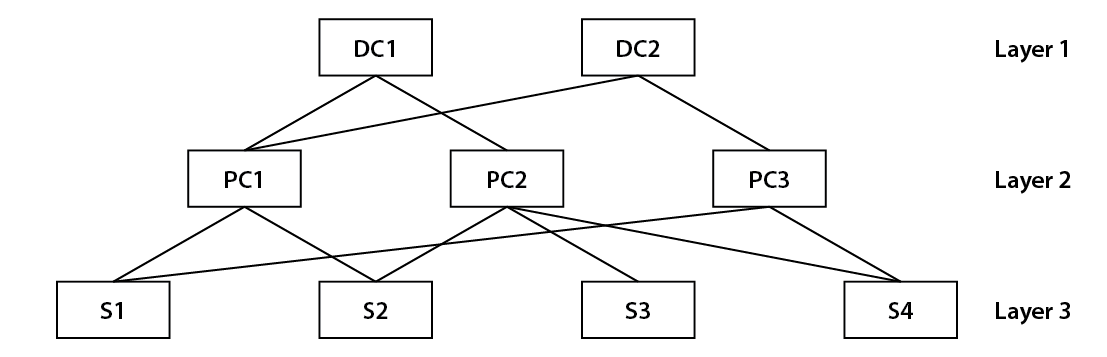
\includegraphics[scale = 0.75, angle = 0]{figures/Formalisation-04}
\caption{Example representation of a belief system with the different layers and several links between the layers.}
\label{fig:Formalisation-04}
\end{figure}

Each issue is categorised by four parameters: the state, the aim, the preference and the awareness. The state defines the view of the agent of a certain i
sue as it is in the real world. This view does not have to match reality and can be influenced by other agents. The aim shows what the agent would like to see hapenning in the world. The preference  which is a derived parameter, defines the importance that the agents places on the different issues. It is calculated depending on the state of the issue, the aim of the agent and the causal relations linked to this issue. The sum of all preference weights on any single layer of the belief tree have to be equal to 1. Finally, the awareness represents the fact that agents are aware of a specific issue or not. It can take the value of 0 or 1. If an agent is not aware of an issue, it will not consider it in any calculation as if it did not exist. The belief tree structure also contains causal relations. These links the issues on the different layers of the structure. These are the representation, in the agent's mind, of how each of the issues are related to each other within the technical model and which issues affect which other issue.

Based on these initial explanations, it is possible to specify the belief tree structure as follows:

\begin{equation}
belieftree = [own_{tree}, others_{tree, n}]
\end{equation}

where $n$ represents the number of agents present in the model.

To further specify the tree of the agent considered, the following can be said:

\begin{equation}\begin{split}
own_{tree} &= [issues_k, causal\text{ }relations_l]\\
issues &= [state, aim, preference, awareness]
\end{split}\end{equation}

where $k$ defines the number of issues present in the belief tree structure and $l$ the number of causal relations.

And it is also possible to specify the structure used to saved the perceived knowledge of the belief of the other agents:

\begin{equation}\begin{split}
other_{tree} &= [issues_k, causal\text{ }relations_l]\\
issues &= [state, aim]
\end{split}\end{equation}

Note that there is no need to calculate the preference of other actors. This is because that is not used within the decision making process of the agents to select a specific action to perform.

In both cases, the issues are specified with deep core issues first, policy cores following and ending with secondary issues. The causal relations are specified in the following example order: DC1-PC1, DC1-PC2, DC2-PC1, DC2-PC2, PC1-S1, PC1-S2, .... The state, preference and causal relation parameters are then specified on the interval of [-1, 1]. The preference is a percentage based parameters and is therefore calculated to be a number on the interval [0, 1].



%\begin{equation}
%issue = < name \times agentOwner \times agentOther \times knowledge \times layer \times S \times A \times P >
%\end{equation}
%
%where $name$ is the unique name of the issue, $agentOwner$ is the agent to which this belief system is associated, $agentOther$ is a list of all other agents present in the model, $knowledge$ defines whether an agent is aware of a certain issue or not, $layer$ represents on which layer the issue is present, $S$ is the state on an interval $[-1, 1]$, $A$ is the agent's aim for this issue on an interval $[-1, 1]$, and $P$ is the preference of an agent on an interval $[0, 1]$.
%
%The \emph{knowledge} parameter is given as a 2-tuple as: \texttt{(status, tick)} where \texttt{status} defines whether the issue is known (value of 1) or not (value of 0) and \texttt{tick} defines when the issue was introduced to the agent if it is known. If an issue is removed from the decision making process, then the value of \texttt{status} will be -1. The \emph{layer} parameter can take three value: 1 for deep core issues, 2 for policy core issues and 3 for secondary issues. The \emph{preference} parameter $P$ is split in two: preference for the agenda setting and preference for the policy formulation. Each takes a value on the interval $[0,1]$, and is calculated in a very similar way but at different points in the simulation. The difference is explained later on.
%
%Note that if $agent \neq agent$, then the data obtained on the beliefs representation of the beliefs of an agent from another agent. This might not be accurate due to partial knowledge sharing. How these are affected is explained later on.
%
%As mentioned earlier, the issues are related through links. These links are causal relations and are the agent's explanation for the current values of the issues. Two types of links are present in the model. Their parameters are given by:
%
%\begin{equation}\begin{split}
%agent \times agent \times issue PC \times issue DC \times CW \\
%agent \times agent \times issue S \times issue PC \times CW
%\end{split}\end{equation}
%
%where $CW$ is the causal weight which is specified on the interval $[-1,1]$ and where $0$ means that there is no causal relation between the two issues.


%- PARAMETERS - The policy network
\subsection{Policy network}

The policy network represent the links between the different agent within a single subsystem. The attributes for these links are given below:

\begin{enumerate}
\item A \emph{policy network link} is represented as a 7-tuple \texttt{link = (agent1, agent2, trust, trustDecay, conflictLevel, temp1, temp2)} where \texttt{agent1} and \texttt{agent2} are the agents at the end of a link, \texttt{trust} is the trust value, \texttt{trustDecay} is the decay value at which the trust diminishes per time interval, \texttt{conflictLevel} is the conflict level characterising the relation between two agents for specific issues and \emph{temp1} and \texttt{temp2} are the parameters used for when an agent is in a team or a coalition.

\item The \emph{trust} value can take three main values. For -1, there is no knowledge for both actors that they know they exist. This means that they cannot network together without external introduction from a third party. For 0, the actors have no connection but know each other exist. Any positive integer relates the value of trust between the two agents. The trust is given on the interval $]0,1]$. Note that trust is relative amongst all links. The policy network links between policy makers can never be -1 as policy makers are public figures. Furthermore, a link cannot be downgraded to -1, it can only start at -1. As the trust decays over time at a specific rate, there are several actions or events that can lead to a growth or stop the decay in the trust between two agents. This is detailed later on.

\item The \emph{trust decay} is represented by a 3-tuple \texttt{(value, initial, time)} where \texttt{value} is the current value of decay which changes depending on the interaction of the agents, \texttt{initial} is the initial value of the trust decay that is a set value set by the modeller initially and \texttt{time} is an integer stating the amount of time intervals left before the value returns to its initial value.

\item The \emph{conflict level} parameter is determined for each agent for each issue's aim and state. Note that the conflict level between two agents will be difference depending on which agents is considered as the conflict level is obtained based on the perception of another agent's beliefs. The conflict level is therefore given as a 2-tuple for each link: \texttt{(agent 1, agent 2)}. Then for each agent, the conflict level is defined per issue for the state and then for the aim. The conflict level is then calculated using:

\begin{equation}\begin{split}
aim \text{ } conflict \text{ } level_{n,n_m} &= |A_n - A_{n_m}| \\
state \text{ }conflict \text{ } level_{n,n_m} &= |S_n - S_{n_m}|
\end{split}\end{equation}

where $A$ is the aim, $S$ is the state, $n$ is the agent for which the conflict level is calculated and $n_m$ is the perceived belief of agent $n$ on agent $m$ for that specific issue.

The resulting value is then formatted into a coefficient to be used in the grading of actions as is shown later on. When the result obtained is between 0 and 0.25, the conflict level is considered to be low, the coefficient is then set at 0.75. When the result obtained is between 0.25 and 1.75, the conflict level is considered to be medium, the coefficient is set to 0.85. Finally for a result higher than 1.75, the conflict level is considered high and the coefficient is set to 0.95. Note that the coefficients values can be varied by the modeller during experimentations.

\item The \emph{temporary} parameter is only used when one of the two agents joins a team or a coalition and is given as a 3-tuple by: \texttt{type, trust, conflictLevel}. The \texttt{type} refers to whether the agent is in a team or a coalition. The \texttt{trust} is calculated as follows. Assume there is a link between \texttt{agent1} and \texttt{agent2}, and that \texttt{agent1} enters a team. Then the trust parameter of the links of all agents within the team with \texttt{agent2} are considered and averaged into one value. This value then becomes the temporary trust parameter for the link. A similar behaviour is considered for the \texttt{conflictLevel} parameter. However, it is not an average that is done but a case by case consideration. If one of these agent has an \texttt{average} conflict level then it is chosen. If this is not the case but there is a \texttt{high} level of conflict, that is taken next and then the \texttt{low} level of conflict is considered.

The temporary parameters are either related to \texttt{agent1} because it joined a team or a coalition or \texttt{agent2}. This means that if both agents join a different coalition, then they will use a different trust level depending on which agent is communicating with the other and considering their presence in a team or a coalition. Furthermore, this will only happen if the agent is communicating on behalf of his team or coalition. In the case of direct agent to agent interaction, then the original trust value is used.

Note that the \emph{temp} parameter is wiped every cycle and reconstructed at the beginning of the team action cycle. This is done to more easily update the trust and conflict level parameters without the need for additional calculation and the need to consider the trust decay parameter. 



\end{enumerate}

%- PARAMETERS - The super policy network	
\subsection{Super-policy network}

This network is modelled on the policy network model. However, it consists of connections only connecting agents which are in different subsystems. The parameters used are similar to the policy network parameters. The \emph{temporary} parameters are however not used as coalition or teams are not considered on cross-subsystem communications.

%- PARAMETERS - The affiliation network
\subsection{Affiliation network}

The affiliation network is a network that looks at the political affiliation of the different actors. Its links are represented as a 3-tuple given by \texttt{(affiliation1, affiliation2, affiCoef)} where \texttt{affiliation1} and \texttt{affiliation2} are the affiliations that are connected by the link and \texttt{affiCoef} represents the influence that an actor with an affiliation 1 can have on an actor with affiliation 2. The \emph{affiliation coefficient} is given on the interval $[0,1]$.

%- PARAMETERS - The system network
\subsection{System network}

The systems network is a network similar with the affiliation network. It is however composed of directed links between the different systems. This network is exclusively used in the context of the diffusion theory. Each link is composed of a 3-tuple write as: \texttt{system1, system2, type)} where \texttt{type} defines the nature of the relationship between the two networks. It can be friendly, dominant, competitive or coercive. More details are provided later on in this chapter.


%- PARAMETERS -  The policy instruments
\subsection{Policy pond and policy instruments}

The policy pond is related to the three streams theory. This pond contains all possible policies which the agents can choose from. Within the scope of this work, there are two types of policies within this pond. They are differentiated by their aggregation level. The main difference between these two types of policies is that the lower level of aggregation policies are then ones that can be implemented as instruments by the agents present in the model. They can therefore also contain feedback effects. The two policy levels are related with parent children relations as shown in \autoref{fig:Formalisation-09}. These relations can be objctive or subjective depending on the theory considered. They represent the amount of relation between the policies on the different level in percentage. The policies are then given as:

\begin{figure}
\centering
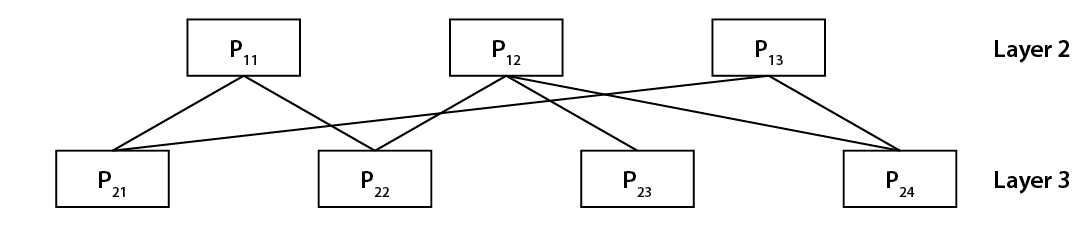
\includegraphics[scale = 0.75, angle = 0]{figures/Formalisation-09}
\caption{Policy pond representation with the two levels of aggregation.}
\label{fig:Formalisation-09}
\end{figure}

\begin{enumerate}
\item A \emph{policy} is represented as a 5-tuple \texttt{(name, impact, change, awareness, feedback)} where \texttt{impact} is related to the impact of the policy on a specific issue, \texttt{change} is the objective change expected in the model due to this policy, \texttt{awareness} is related to the avalability of the policy for a specific agent and \texttt{feedback} is related to the expected model feedback from the implementation of the policy considered.

\item The \emph{impact} of a policy instrument is given as a 2-tuple: \texttt{(issue, impact)} where \texttt{issue} defines which of the issues is affected and \texttt{impact} specifies by how much. For higher level instruments, the issues are the policy core issues while for the lower level instruments, the issues considered are the secondary issues. The values for the impact are subjective and can be influenced by the agents in the model. 

\item The \emph{change} due to a policy instrument is the subjective representation of the impact of the policy instrument. These are the actual changes that will occur in the model with the implementation of the instrument. They are defined by the modeller and cannot be influenced by the agents present in the model. The structure of the parameter is similar to the \emph{impact} parameter. Note that it is for the modeller to normalise all changes of all policy instrument if these policies are policies that apply on different durations. The way the instruments are graded is the same for all and does not take into account the time over which the policy instrument is to be implemented.

\item The \emph{awareness} parameter defines whether a certain policy instrument is known in a subsystem. It is therefore defined as a list of 2-tuple: \texttt{(subsystem, awareness)} where \texttt{subsystem} defines which subsystem is concerned and \texttt{awareness} defines whether this policy instrument is known in the subsystem by taking the value 0 or 1.

\item The \emph{feedback} parameter defines what additional feedback can be expected from the measure. The feedback can be placed into three main categories: impact on the electorate composition, impact on the knowledge of the belief tree, impact on the resource allocation for policy entrepeneurs. These are related to the feedback theory.

In the case of impact on the electorate composition, certain policy instruments will lead to changes to the \texttt{electorate.representation} parameter. This change in turn will lead to the recalculation of the resources attributed to the policy makers.

For the impact on the knowledge of the belief tree, it is the $issue.knowledge$ parameter that can be affected. Specific policy instrument can place certain issues out of reach of the decision making process. They would then take the \emph{knowledge} value of -1.
\end{enumerate}



%- PARAMETERS - The agenda parameters	
\subsection{Agenda}

The \emph{agenda} is a 2-tuple given by \texttt{agenda = (problem, policy)} where \texttt{problem} is the problem chosen to be on the agenda, \texttt{policy} is the policy chosen to be on the agenda. Note that there is one agenda per subsystem. Furthermore, the agenda policy is not required in all theories considered. The policy appears on the agenda only when considering the three streams theory. This is elaborated on later on in this chapter.

%- PARAMETERS - The teams
\subsection{Teams}

The teams are created following the three streams theory.  They contain a number of agents that feel they share their beliefs for a specific issue. A team is therefore given as a 6-tuple written as: \texttt{(team ID, lead, members, issue, creation, resources)} where \texttt{lead} is the leader of the team (the agent that created the team), \texttt{members} is the list of members that are part of the team, \texttt{issue} is the policy issue that the team is advocating for, \texttt{creation} is the time at which the team has been created and \texttt{resources} consists of the resources at the disposal of the team to perform actions. The resources are calculated as the sum of all the members belonging level. It is therefore a number that can be above 1.

%- PARAMETERS - The coalitions
\subsection{Coalitions}

\textcolor{red}{This will probably be updated later.}


%- PARAMETERS - The external events
\subsection{The external events}

The external events that are considered are external events that affect the policy emergence model. External events that would affect the technical model such as a flood for a hydrological technical model are of no interest and considered out of scope of this report. However, the impact on the model such as a change in the electorate composition due to a high amount changes due to the flooding is of interest.

The following is a non-exhaustive list of potential external events which the modeller could use.

\begin{enumerate}
\item An election - this would create a change in the \texttt{electorate.representation} parameter which would in turn lead to different resources allocation for the policy makers.
\item The introduction of a new issue - a new issue could be introduced to the system or to a subsystem. This would affect the \texttt{agent.knowledge} parameter for all agents present in the model.
\item Resources shift - a shift in the resources distribution due to an external event could be modelled. The \texttt{agent.resources} parameter would be changed.
\item Policy network shifts - change in the trust parameter.
\item Affiliation network shift - change in the \texttt{affiCoef} parameter.
\end{enumerate}

%%%%%%%%%%%%%%%%%%
%%%%% THE CYCLE %%%%%
%%%%%%%%%%%%%%%%%%
\section{The model cycle}
\label{sec:modelCycle}

This is the cycle iterated through when the entire model is considered. Different theories are related to the different parts of the model and are mentioned below:

\begin{enumerate}
\item Tick initialisation:
	
	\begin{enumerate}
	\item \emph{World simulation:} The technical simulation which is an exogenous party to the model or an internal technical model are run to provide inputs for the next step.
	\item \emph{Trigger of external events:} Any event that the modeller decides to implement are activated at this stage of the model cycle.
	\item \emph{Update of the truth agent:} The technical output is converted into normalised data fitting with the issues present in the belief tree. These are placed in the truth agent's $S$ parameters.
	\item \emph{Electorate action:} The electorate influences the belief of the policy makers.
	\item \emph{External parties belief update:} External parties update their $S$ for the issues for which they are interested in. They update with the truth agent's beliefs.
	\item \emph{All agents belief update:} The rest of the agents which are not external parties or the truth agents have their beliefs updated. The external agents share their beliefs with the policy makers and entrepreneurs. This sharing of information is affected by the affiliation of the different agents.
	\end{enumerate}
	
\item Agenda setting:

	\begin{enumerate}
	\item \emph{Agent issue classification and selection:} Each agent ranks his deep core and policy core beliefs. The agent then selects an issue that he will advocate for in his policy core beliefs based on his ranking.
	\item \emph{Creation of the coalitions (ACF):} Agents are set up in different coalitions according to their deep core beliefs. This step only occurs within the context of the advocacy coalition framework.
	\item \emph{Deliberations (Backbone+/3 Streams/ACF):} All agents deliberate and perform their actions. The deliberations do not occur when considering the backbone model. The details for each model are provided in later sections.
	\item \emph{The policy makers rank the issues:} Each policy maker updates his preferences for his deep core and policy core beliefs. This is to take into account the effects of the deliberations and influencing from the other agents.
	\item \emph{Agenda setting:} The system calculates the systemwide grades of the issues chosen by the different policy makers. They are then ranked and the issue at the top of the ranking is selected to be the agenda. This constitutes the agenda with which the policy formulation process will work.
	\end{enumerate}
	
\item Policy formulation:

	\begin{enumerate}
	\item \emph{Policy pool selection:} Based on the issue selected from the agenda, each agent can select a certain number of secondary issues they belief will have an impact on the issue on the agenda. Related to these secondary issues, they can determine a set of policy instruments that would have an impact on the issue on the agenda through their secondary issues. 
	\item \emph{Policy instrument selection:} Each agent selects a policy instrument that he will be advocating for during the policy formulation based on the set of policy instruments available to them.
	\item \emph{Creation of the coalitions (ACF):} Agents are set up in different coalitions according to their deep core beliefs. This step only occurs within the context of the advocacy coalition framework.
	\item \emph{Deliberations (Backbone+/3 Streams/ACF):} All agents deliberate and perform their actions. The deliberations do not occur when considering the backbone model. The details for each model are provided in later sections.
	\item \emph{The policy makers rank the instruments:} Each policy maker upgrades their policy instrument preferences after the deliberation phase.
	\item \emph{The system decides if a policy instrument should be implemented:} The system checks if the consensus threshold is being met. If it is, the policy instrument is implemented into the world simulation and removed from the model.
	\end{enumerate}
	
\item \emph{The model advances to the next time step:} The clock is advanced to the next tick. End of ticks actions are also performed.

\end{enumerate}



%% THE BACKBONE
\section{The backbone model}

The backbone model refers to the smallest model used to simulate the emergence of policies. This model does not contain any of the theories found in the literature and is built in two main parts. In the first part, the agenda setting part, where the policy makers grade the issues according to their view of the world and decide on a policy and a problem to tackle. Next, in the policy formulation process, these same policy makers select a policy instrument based on their beliefs. If they meet the number of policy maker threshold for implementation, the instrument is implemented. Within this backbone model, the agents do not communicate with each other. The backbone model also contains the electorate agents. These can influence passively the policy makers as is shown in the algorithms shown below. The electorate feature can be turned on and off depending on the experiment or verification that is being performed on the model.

%-
\subsection{The backbone policy cycle}

The backbone policy cycle is presented below. The steps that were already mentioned in detail previously are not re-explained.

\begin{enumerate}
\item Tick initialisation:
	\begin{enumerate}
	\item \emph{World simulation}
	\item \emph{Trigger of external events}
	\item \emph{Update of the truth agent}
	\item \emph{Electorate actions}
	\item \emph{External parties states update}
	\item \emph{All agents states update}
	\end{enumerate}
\item Agenda setting:
	\begin{enumerate}
	\item \emph{Agents deep and policy core issues preference update}
	\item \emph{Agent issue classification and selection}
	\item \emph{Agenda setting}
	\end{enumerate}
\item Policy formulation:
	\begin{enumerate}
	\item \emph{Agents secondary issues preference update}
	\item \emph{Policy pool selection}
	\item \emph{Policy instrument selection}
	\item \emph{The system decides if a policy instrument should be implemented}
	\end{enumerate}
\item \emph{The model advances to the next time step}
\end{enumerate}

%-x
\subsection{Tick initialisation}

This section presents the different algorithms required to appropriately initialise each tick in the model.

%0
\paragraph{Agent beliefs update}

All agents must been updated on the different issues' progress based on the world simulation and the information that the external parties have gathered. These updates are based on the affiliations of the agents and the external parties they are communicating with. For each agent, the updated beliefs of the agents are given by:

\begin{equation}
S_{agent} := S_{agent} + \frac{1}{n} \sum_{i=1}^n \left( \left(S_{EP_n} - S_{agent} \right) \cdot affiCoef_n \right)
\end{equation}

where $S$ stands for the issue state, $EP$ stands for external parties and $affiCoef_n$ is the affiliation related weight. The affiliation coefficient is the one that relates the affiliation of the agent and the affiliation of the external party selected.

%0
\paragraph{Electorate action on policy makers}

\textcolor{red}{How the electorate are updated from the truth agent has yet to be formalised and introduced in the code. Right now, the electorate is an agent with a static belief.}

The policy makers are passively influenced by the electorate. Each electorate has a certain affiliation to which policy makers are also related. Each policy makers' issues will therefore be influenced by their respective electorate. This happens as a passive effect where the issue aims of the policy makers slowly progress towards the issue aims of the electorate. The gap is introduced in the equation to mark a sense of urgency. The equation to calculate the change in the aim of the policy maker is given as follows:

\begin{equation}
A_{PM} := A_{PM} + \left(A_{El} - A_{PM} \right) \cdot 0,001 \cdot \left| A_{El} - S_{El} \right|
\end{equation}

where $El$ stands for electorate and $PM$ for policy maker. Note that this is only performed for the issues of the policy maker for agents with matching affiliations.


%-
\subsection{Agenda setting}

This section presents the different algorithms that are used to set the agenda and obtain an issue at the end of this step.

%0
\paragraph{Preference calculation update (deep and policy core issues) - Policy makers and entrepreneurs}

The preference parameter for the beliefs of the agents defines which issue the agent will want to address first. This parameter is calculated for all issues present in the belief tree. Within the context of the agenda setting, the preference is only calculated for the deep core and policy core beliefs.


% It is however calculated differently for the agenda setting process and the policy formulation process. Similarly depending on which layer the issue is in, the calculation might be affect. 

To calculate the preference for all of the deep core issues per agent, the gap between the state and the aim is calculated for each issue. It is then normalised amongst all deep core issues to formulate the preference. The equation is given as follows:

\begin{equation}
P_i = \frac{ |A_i - S_i|}{\sum_{j=1}^n |A_j - S_j|}
\end{equation}

where $j$ is defined at the number of deep core issues and $i$ characterises the deep core issue being selected for the calculation.

For the policy core, a similar approach is being used. The main difference resides in the fact that there are causal relations that should also be taken into account. These causal relations are not always helping bridge the gap between the aim and the state of an issue. If they do not, they must then be discarded. To calculate the new preference, the gap for the issues is considered along with the impact of the causal relation on the gap of the issues on the above layer. Once again, all the preferences on one layer must be normalised. The resulting equation that can be used to calculate the preference is given by:

\begin{equation}\label{eq:preference2}
P_k= \frac{ |A_k - S_k| + \sum_{j=1}^n |CW_j \left( A_j - S_j \right)|}{\sum_{l=1}^p \left[ |A_l - S_l| + \sum_{j=1}^n \left|CW_{j,l} \left( A_{j,l} - S_{j,l} \right) \right| \right]}
\end{equation}

The sums only include these terms if $CW_j$ and $\left( A_j - S_j \right)$ have the same sign. If it is not the case, these terms are not considered. And where $p$ is defined at the number of policy core issues, $k$ characterises the policy core issue being selected for the calculation, $j$ specifies the associated deep core and $CW$ represents the weight of the causal relation.

Note that \autoref{eq:preference2} also applies to the secondary issues but with everything considered one layer lower.


%0
\paragraph{Selection of the issue (agent)}

For the selection of the issue for whith the agent will advocate for, the policy core issues are considered. All policy core issues are ranked based on their preference value as shown earlier. The highest preference is chosen for each agent.

%0
\paragraph{Policy ranking and selection (system) (1)}

To constitute the agenda, an issue has to be chosen for the entire subsystem. For this two methods are proposed which can yield different results. The first method considers all the top issues as graded by the agents. They are affected by the normalised resources of the agents. The grade of each issue is the sum of all agent's resources which have chosen that issue as their top issue. Whichever policy has the highest grade becomes the policy that will be chosen for the agenda.

%0
\paragraph{Policy ranking and selection (system) (2)}

The second method used for the ranking and selection of the issues is similar to the first one. The difference is that here all issues are taken from each agents. They are then weighted all together and not simply the issues at the top of the ranking of each agent. This approach is meant to represent a different approach to the power dynamics in the model. The grade for each policy is then obtained as:

\begin{equation}
rankingGrade = \sum_{i=0}^n \left( \frac{1}{P_{rank}} \cdot resources_n \right)
\end{equation}

where $n$ is the number of agents and $P_{rank}$ is the ranking of the policy for that agent.

The issue with the highest grade is then taken as the issue for the agenda.


%-
\subsection{Policy formulation}

This section presents the different algorithms that are used within the policy formulation step.


%0
\paragraph{Preference calculation update (secondary issues) - Policy makers and entrepreneurs}

Within the context of the policy formulation, the secondary issue preferences have to be selected. The equation and the procedure are very similar to the calculation for the policy core issues in the agenda setting. The main different is that only issues that are related to the issue on the agenda are considered within the belief tree. Any secondary issue that is not related to the issue on the agenda is discarded and considered to be irrelevant to the agents.

Once again, the equation used to calculate the secondary issue preferences are given by: 
\begin{equation}
P_k= \frac{ |A_k - S_k| + \sum_{j=1}^n |CW_j \left( A_j - S_j \right)|}{\sum_{l=1}^p \left[ |A_l - S_l| + \sum_{j=1}^n \left|CW_{j,l} \left( A_{j,l} - S_{j,l} \right) \right| \right]}
\end{equation}

The sums only include these terms if $CW_j$ and $\left( A_j - S_j \right)$ have the same sign. If it is not the case, these terms are not considered. And where $p$ is defined at the number of secondary issues, $k$ characterises the secondary issue being selected for the calculation, $j$ specifies the associated policy core and $CW$ represents the weight of the causal relation.

%0
\paragraph{Policy instrument pool construction}

At the beginning of the policy formulation, a pool of policy instrument needs to be established based on the agenda. For this pool, all policy instruments that have an impact on a secondary issue without preference 0 are considered. The agent will then be able to select any policy instrument for that pool and to promote it to other agents during the policy formulation process.

%0
\paragraph{Policy instruments ranking and selection (agent)}

During the policy formulation step, the agents must chose their preferred policy instruments from a pool of preselected policy instruments. For this, the agents look at the preference of the secondary issue (calculated previously) and adjust this preference with the expected impact of the policy instrument. The equation used to calculate the grade of each policy instrument is given by:

\begin{equation}
G_i = \sum_{j=1}^n \left[ impact_j \cdot \left( A_j - S_j \right) \cdot P_j \right]
\end{equation}

where $n$ is the number of impacts this policy instrument has, and $j$ represents the secondary issue and the associated impact of the policy instrument on that issue.

Note that an instrument is only considered if its impact is of the same sign as the gap. If this is not the case, the instrument will be counter productive in the mind of the agent and should therefore not be implemented. The grade assigned is then 0.

%0
\paragraph{Consensus check 1 - Unanimity}

This check consists of checking whether all instrument chosen as the top instrument by the policy makers are the same. This is done by checking the \texttt{agent.advocacy.polins} parameter. If this is the case, the policy instrument can be implemented

%0
\paragraph{Consensus check 2 - Majority}

The majority check is similar to the previous. Here however, the check consists at counting how many time each issue in the \texttt{agent.advocacy.polins} parameter there are. If the count is larger than half the number of policy makers plus one, then the policy instrument can be implemented.


%% THE BACKBONE + MODEL
\section{The backbone+ model}

The section presents the backbone+ model. This model uses the backbone model architecture but adds the policy network along with individual agent actions. This backbone+ model is an artifact of the formalisation from the conceptualisation. In strict terms it does not address a single policymaking theory in itself but helps build to all four theories addressed in this report. The items that are similar to what was presented in previous sections are not re-explained. The additional parts are detailed.

%-
\subsection{The backbone+ policy cycle}

Each agent has a certain number of actions that (s)he can perform. Within the cycle presented earlier, these actions can be performed at the deliberations stage. An algorithm is devised for the agent to decide which actions to perform.  This is shown below in details. Note that the deliberations for an agent end after all its initial resources are exhausted. The deliberation phase algorithm is the same for the agenda setting process and the policy formulation process. The main difference is the set of options that are available to the agents in each of the phases. For the agenda setting process, both the issue selected by each agent is discussed, this means that agents can perform actions on the selected issue and the related causal relations. In the policy formulation process, the agenda is already set. Agents must first select a secondary issue they will advocate for and hence a policy instrument. The action then performed are all related to either the secondary issue selected or the causal relations that relate to this issue. Agents can therefore only perform actions on issues and causal relations that are related to the agenda policies and problems and to the policy instrument they have each selected.

\begin{enumerate}
\item Tick initialisation:
	\begin{enumerate}
	\item \emph{World simulation}
	\item \emph{Trigger of external events}
	\item \emph{Update of the truth agent}
	\item \emph{Electorate actions}
	\item \emph{External parties belief update}
	\item \emph{All agents belief update}
	\end{enumerate}
\item Agenda setting:
	\begin{enumerate}
	\item \emph{Agent issue classification and selection}
	\item \emph{Deliberations:}
		\begin{enumerate}
		\item \emph{Resources receival:} The agent receives its resources based on modeller-specific data.
		\item \emph{Policy network upkeep or maintenance:} The agents perform actions that will either renew or maintain a policy network link. A part of the agent's resources are spent for this process. Agents can have one of two strategies: largest network strategy and focused network strategy. The strategy used by each agent is chosen by the modeller.
		\item \emph{Individual belief actions:} These actions are the actions that have an impact on the belief of the other agents directly or indirectly. The agents use all their remaining resources to preform these actions. For the external parties, these actions consists of blanket framing and electorate influence. For the policy makers and entrepreneurs, these actions are framing, and influence on state and aim of the issue they advocate for. These actions and how which is selected is detailed later on.
		\end{enumerate}
	\item \emph{The policy makers rank the issues}
	\item \emph{Agenda setting}
	\end{enumerate}
\item Policy formulation:
	\begin{enumerate}
	\item \emph{Policy pool selection}
	\item \emph{Policy instrument selection}
	\item \emph{Deliberations:}
		\begin{enumerate}
		\item \emph{Resources receival}
		\item \emph{Policy network upkeep or maintenance}
		\item \emph{Individual belief actions:} The actions here are similar to the actions during the agenda setting process. The main difference is that these actions are focused on the secondary issues instead of the policy core issues as these are the issues that the agents are advocating for.
		\end{enumerate}
	\item \emph{The policy makers rank the instruments}
	\item \emph{The system decides if a policy instrument should be implemented}
	\end{enumerate}
\item \emph{The model advances to the next time step}
\end{enumerate}

%-
\subsection{Backbone+ model related algorithms - networks}

This section details all the additional algorithms that are required for the backbone+ model related to the policy network. There is 20\% of the resources for the agenda setting process that is reserved for the agent to spend on network maintenance. The agents are allowed to five actions each time spending 4\% of the total amount of resources for each action. The order in which agents are selected to perform their network actions is random.

The two strategies that can be used for the maintenance of the network of an agent are mentioned below:

\begin{enumerate}
\item Largest network strategy - the agent will look into increasing its network as much possible:
	\begin{enumerate}
	\item The agent first wants to keep all links active. Any link that is below 30\% trust level will be targeted for action. The lowest, but still above 0, will have priority.
	\item If all links are above 30\% trust, the agent will look into introducing new links which had 0\% trust. The priority is placed on the link with agents with the closest beliefs.
	\item If there are still resources left after step 1 and 2 are complete, the agent will maintain the link with the lowest trust level in the network.
	\end{enumerate}
\item Focused network strategy - the agent will focus on maintaining a network of agent sharing its beliefs: (note that when it is stated similar belief, this relates to the problem that the agent is advocating for and no other issue)
	\begin{enumerate}
	\item The agent will look first for link where an agent with a similar belief (one of the agents has his belief within 0.2 of the other agent's aim belief) or higher belief level and with a trust which is lower than 70\%. The agent will prioritise based only on the trust level as long as the belief criteria is met.
	\item If no link qualifies, then the agent will seek to introduce new links in his network. The agent will select agents that have a similar belief or higher belief level.
	\item If both step 1 and 2 are met, the agent will look into maintaining a trust level above 70\% for links still in service. The priority is put on the links with the lowest trust value.
	\item If all previous steps are met, then the agent will simply look for new links.
	\end{enumerate}
\end{enumerate}

The actions described above are explained in more details below.

%0
\paragraph{Maintaining the trust in a network}

An agent can increase the trust in a network link if he feels the trust level is too low. This trust maintenance is dependent on three main parameters: the resources spent and the affiliation of both agents. The total increase in trust for such an actions is calculated as:

\begin{equation}
trust := trust + resources \cdot affiCoef
\end{equation}

where the $affiCoef$ is the weight related to the affiliation of the two agents. If they share the same affiliation, then it is equal to 1.

%0
\paragraph{Establishing a new network link}

Agents can also establish links with other agents for which they know they exist. This action can only be performed when the \texttt{link.trust} parameter is equal to 0.

If this is the case, then the trust can be increased through the spending of resources. The new trust level is then calculated similarly to the trust maintenance but with a small malus to account for the initial investment costs. The equation is given as follows:

\begin{equation}
trust := resources \cdot affiCoef \cdot 0.5
\end{equation}

%0
\paragraph{Seeking agents of similar beliefs}

Similar beliefs are defined on the aim of an issue being advocated for at the policy core level. There are several steps to seek agents with similar beliefs:

\begin{enumerate}
\item Seek all links with trust equal to 0 or higher and select their associated agents.
\item Select the aim parameter of the problem of the original agent.
\item For each associated agent, check its aim parameter for this same problem issue.
\item Calculate the difference of the parameter between the original agent and the associated agent for this issue.
\item Rank all differences from lowest to highest where the lowest is considered to be an agent of similar beliefs.
\end{enumerate}

This ranking is impacted by partial knowledge of the original agent on the associated agent's beliefs.

%-
\subsection{Backbone+ model related algorithms - external parties actions}

This section details all the additional algorithms that are required for the backbone+ model related to the actions of the external parties. Out of all the resources reserved for external parties, 50\% of these resources are devoted to blanket framing while 50\% are devoted to electorate influence. These are each spent in interval of 10\% of the total amount of resources dedicated to these actions. This means that overall, each external party will perform five blanket framing actions and five electorate influence actions.

%0
\paragraph{External parties - Blanket framing}

The external parties can perform framing tasks. The framing expressed by these parties is called blanket framing as it impacts all of the agents present in a subsystem at once. This framing is focused on influencing all of the causal relations related to the issue that was selected by the external party performing the action. Its impact is dependent on affiliation and on the resources that the external party is spending. For each causal relation, the external party checks the impact of performing a framing action for all agents present in the model. This is based on his partial knowledge of other agent's belief on the causal relation. The grades are calculated as follows:

\begin{equation}\begin{split}
G_{cr,m} &= \left| \left(CW_{n} - CW_{n_m} \right) \cdot affiCoef_n \cdot resources \cdot \frac{1}{agents} \right| \\
G_{cr} &= \sum_{m = 1}^{agents-1} \Delta G_{cr, m}
\end{split}\end{equation}

where $cr$ is the causal relation selected, $n$ the external party performing the framing, $m$ the affected agent considered, $nagents$ the total number of agents and $CW$ the causal weight.

The action on a causal relation for which the grade is the highest is then selected to be implemented. The causal relation of the affected agents are then given by the following equation:

\begin{equation}
CW_{m} := CW_{m} + \left(CW_{n} - CW_{m} \right) \cdot affiCoef_n \cdot resources \cdot \frac{1}{nagents}
\end{equation}

Note that this time, the actual causal weight of the causal relation is used and not the perceived one.

\textcolor{red}{Not yet sure how to address this action with the new grading options. The action chosen could be based on the number of agents that prefer the issue of the external party after the action has been performed. This would require counting the number of agents that have for main issue the issue of the external party and the number of them that have it as a seccond choice and so on. If the situation is improved, then that action is selected.}

%\textcolor{blue}{[Note that there is a looming problem with this action as even if its resources are 1, the action will have a very limited impact if there 200 agents for example. To counter this, the modeller might be allowed to inrease the maximum resources to a number above 1 for specific rare events or a weight should be added depending on the total number of agents present in the model.]}

%0
\paragraph{External parties - Electorate influence}

The external parties can influence all the electorate's aims directly. The external party will only select the aim of the issue for which he is advocating for. The external party performs the action in his head using the following equation and his full knowledge of the other agent's beliefs:

\begin{equation}
A_{El, i} := A_{El, i} + \left(A_{n, i} - A_{El, i} \right) \cdot affiCoef_n \cdot \frac{resources}{nEl}
\end{equation}

where $n$ is the external party, $i$ is the issue and $nEl$ is the number of electorates. Note that for this action, it is assumed that the external parties know the aim value of the each electorate for each issue.

Then the external party will proceed to evaluate the preference of the agent influenced based on his partial knowledge of the other agent's belief. This is done for all actions and the grade assigned to each action is the absolute value of the difference between the aim of the external party influencing and the new aim of the agent being influenced. All of these grades are then added for each agent. The grade that is the smallest means that the action lead to agents becoming closer to the external party. The acton is therefore chosen to be implemented.

For the action chosen, the same equation is chosen. Because the external parties have full knowledge of the electorate's beliefs, there is no partial knowledge used and the expected results of the action will be the same as the actual results. 

%-
\subsection{Backbone+ model related algorithms - policy makers and entrepreneurs actions}

This section details all the additional algorithms that are required for the backbone+ model related to the actions of the policy makers and entrepreneurs. For each round of actions, the agent can spend 10\% of the total amount of resources reserved for the belief actions. This means taht the agent can perform ten actions in total. For each round, the agent considers all actions mentioned below. Each of these actions is graded and then the action with the highest grade is chosen to be implemented.

\emph{After each action has been performed by one agent, the model randomly selects an agent and performs all these steps again until that new agent has performed his action. This continues until all agents have spent all their resources.}

The equation to calculate the grade of each action and the one used to implement the actions are different. The first difference is that one will use partial knowledge of the other agent's belief while one uses the actual beliefs. The second difference is the introduction of the conflict level for the grading of an action. This parameter stems from the ACF theory and is a parameter that is used to describe the likelihood of two actors discussing on a specific topic. For average level of conflict, they are more likely to talk to each other for example. This parameter is not used for the implementation of the actions. Finally, a parameter is used for purposes of experimentation. This parameter is used to help facilitate the influence of policy makers. This is because they are the decision makers and could therefore be considered prime targets to get issues faster on the agenda for the agents in the model. For this, the actions affecting the policy makers can be weighed up compared to the actions of the policy entrepeneurs. This parameter can be varied by the modeller during testing to see what affects most the policy emergence process. It should be situated on the interval $[0,1]$. It is once again only used in the grading equation and not for the implementation.

%0
\paragraph{Individual action - Individual framing}

The different agents can attempt to influence the causal relation belief of other agents. This framing action is similar to the blanket framing action of the external parties but applies to only one agent. Within the context of the agenda setting process, agents can perform framing actions on all causal relations related to the policy core they have selected.  For the policy formulation, the causal relations considered are the ones related to the secondary issues selected which are influenced by the policy instrument selected. The change in the causal relation is obtained as follows:

\begin{equation}
CW_{n_m} := CW_{n_m} + \left(CW_{n} - CW_{n_m} \right) \cdot resources \cdot trust_{n,m} \cdot actionWeight
\end{equation}

where $n$ is the agent performing the action, $m$ is the agent on which the action is performed.

Once the estimated new causal relation is obtained, the difference between it and the old causal relation is calculated and set as the grade for this action.

If a framing action is considered to be the best possible action, the following equation is used to implement that decision:

\begin{equation}
CW_{m} := CW_{m} + \left(CW_{n} - CW_{m} \right) \cdot resources \cdot trust_{n,m}
\end{equation}

%0
\paragraph{Individual action - Aim change}

Similarly to framing, agents can attempt to influence the aim of other agents. This is can be done during personal conversation and is therefore impacted by resources, trust and conflict level. The equation to calculate such change is given below:

\begin{equation}
A_{n_m} := A_{n_m} + \left( A_{n} - A_{n_m} \right) \cdot resources \cdot trust_{n,m} \cdot conflictLevel \cdot actionWeight
\end{equation}

where $n$ is the agent performing the action, $m$ is the agent on which the action is performed.

Once again, to provide a grade to this action, the potential new aim is compared to the former aim of the agent.

If this action is selected, the following equation is then used to implement that action:

\begin{equation}
A_{m} := A_{m} + \left(A_{n} - A_{m} \right) \cdot resources \cdot trust_{n,m}
\end{equation}

Note that this action's set of possible issue is different between the agenda setting and the policy formulation processes. In the first, only the policy core issue which was selected by the influencing agent can be used for actions. During the second, only secondary issues related to the policy instrument selected by the influencing agent can be used for the action. This is also true for the next action, the state change.

%0
\paragraph{Individual action - State change}

Finally, similarly to the framing and aim change, agents can attempt to influence the view of the world of other agents through direct interaction. This is the state change action. This is once again done similarly to the other actions, through resources and is impacted by the trust and the conflict level between the agents.

The change is given by the following equation:

\begin{equation}
S_{n_m} := S_{n_m} + \left(S_{n} - S_{n_m} \right) \cdot resources \cdot trust_{n,m} \cdot conflictLevel \cdot actionWeight
\end{equation}

where $n$ is the agent performing the action, $m$ is the agent on which the action is performed.

The grade provided is the difference between the potential new state and the former aim of the agent.

If this action is selected, the following equation is then used to implement that action:

\begin{equation}
S_{m} := S_{m} + \left(S_{n} - S_{m} \right) \cdot resources \cdot trust_{n,m}
\end{equation}

%-
\subsection{Partial knowledge updates}

As mentioned previously, each agent has a certain perception of the beliefs of all other agents in the model on each of the issues state and aims, and on the causal relations. This perception is updated every time an agent performs another action with a fellow agent. Depending on the action performed, each of the agent will gain knowledge about the other agents belief with a certain amount of randomness.

For blanket framing actions, the belief will be shared with a $\pm$ 0.25 randomness on the actual value. For framing, state and aim influence actions, the shared belief is associated with a $\pm$ 0.1 randomness value.

%% THE BACKBONE WITH 3 STREAMS
\section{Backbone model with three streams theory}

This section presents the model of the backbone and the backbone+ model combined to the three streams theory. The three streams theory brings the notion of the coupling of the policy stream, problem stream and politics stream. In the model, this require the addition of several elements. For this, the policy pond is more extensively used. For this model, in both the agenda setting and the policy formulation, the agent can choose a policy from the policy pond and can choose a problem. The problems are based on the belief tree and are defined in preference based on the gap between aim and state for each of the issues presented in the belief tree. Each agent can then choose from both policies and problems. A similar approach is used for the policy formulation.

Furthermore, in the spirit of the policy entrepreneurship model, teams are also added to the three streams model. This teams are used to accelerate the policy learning within the system. These teams can perform similar actions to the actions that each individual actions can perform.


%-
\subsection{The three streams policy cycle}


The new policy cycle used for the three streams theory is presented below. Only the additional parts are detailed.

\begin{enumerate}
\item Tick initialisation:
	\begin{enumerate}
	\item \emph{World simulation}
	\item \emph{Trigger of external events}
	\item \emph{Update of the truth agent}
	\item \emph{Electorate actions}
	\item \emph{External parties belief update}
	\item \emph{All agents belief update}
	\end{enumerate}
\item Agenda setting:
	\begin{enumerate}
	\item \emph{Agent issue classification and selection:} The agent can select from policies or problems their issue.
	\item \emph{Deliberations:}
		\begin{enumerate}
		\item \emph{Resources receival}
		\item \emph{Agent-Team actions:} Each agent can decide to join or start a new team depending on his belief and his choice of policy or problem. Teams are constituted of members that share their beliefs on a policy or a problem. Related to these teams, several actions are performed such that the team will disband in the required circumstances. This is detailed later on.
		\item \emph{Team actions:} When an agent is in a team, he will participate resource-wise to the team. This allows the team to influence agents that are outside of the team such that they align their beliefs to the team's beliefs. The team will also perform actions on its own members in such a way that the agents will have more coherent beliefs. 
		\item \emph{Policy network upkeep or maintenance}
		\item \emph{Individual belief actions:}  Needs details ... (added actions)
		\end{enumerate}
	\item \emph{The policy makers rank the issues}
	\item \emph{Agenda setting}
	\end{enumerate}
\item Policy formulation:
	\begin{enumerate}
	\item \emph{Policy pool selection:} The way the policy pool is defined is different within the context of the three streams theory. This is detailed later on.
	\item \emph{Policy instrument selection:}  Similarly, the policy instrument selection is different for this theory. This is also detailed later on.
	\item \emph{Deliberations:}
		\begin{enumerate}
		\item \emph{Resources receival}
		\item \emph{Agent-Team actions:} Needs details ...
		\item \emph{Team actions:} Needs details ...
		\item \emph{Policy network upkeep or maintenance}
		\item \emph{Individual belief actions:}  Needs details ... (added actions)
		\end{enumerate}
	\item \emph{The policy makers rank the instruments}
	\item \emph{The system decides if a policy instrument should be implemented}
	\end{enumerate}
\item \emph{The model advances to the next time step}
\end{enumerate}



%\begin{enumerate}
%
%\item \emph{Agent-Team actions:} Each agent goes through all agent-team actions which are related to the joining, creating or leaving of a team. Each agent can only be part of one team at a time in the agenda setting process and the policy formulation process. Note that all actives agents can be part of teams. These are the policy makers, policy entrepreneurs and external parties.
%
%	\begin{enumerate}
%	\item \emph{Belonging parameter update:} If an agent is in a team, then its \texttt{agent.team.belonging} parameter is updated based on the latest beliefs. 
%	\item \emph{Leave a team:} An agent will leave a team of his own accord only for one reason: if the belonging level drops below 30\%. If the agent leaves the team he was part of, the team must then be checked to see if it has enough members. If it has less than three members it will have to be disbanded and all agents present in the team are removed from it.
%	\item \emph{Disband the team:} If the agent is the lead of the team, there is a possibility that he will disband the team. This happens when the policy issue the agent is advocating for changes and does not match the issue of the team anymore. This is not checked every tick but every five ticks. If they do not match, the team will be disbanded and all agents removed from the team. The requirements used to create a team are also rechecked every five ticks to see if the members should still be in the team. If the number of members falls below three during this review process, then the team wil be disbanded.
%	\item \emph{Join a team:} If the agent is not in a team, he will first try to join an existing team. For each team considered, he will spend a small amount of resources to gather information. If the gap in his beliefs is above the required threshold for the issue that the considered team is supporting, and his state belief are closed enough to the team's leader state belief on that issue, then the agent can join the team.
%	\item \emph{Create a team:} If the agent has not managed to join a team, then he has the possibility to create a team himself. For this the agents looks towards the agents to which is is connected and has trust. For each of these agents, and considering the policy issue he is advocating for, the agent considers the gap in this issue along with the state to see if he shares beliefs with the other agents. Considering each agents costs a little resources for both the agent searching and the agents he is interacting with. Then depending on the personal strategy of the agent, the agent creates a team with all the agents he has found or he creates a team once he has found a sufficient amount of agents. Note that the gap amount is dependent on the situation along with the state. This is detailed later on.	
%	\end{enumerate}
%	
%\item \emph{Team actions:} The belief actions are split in two parts: the intra-team actions and the inter-team actions. Each part uses 50\% of the resources available to the team in five steps of 10\%. The resources available to team are equal to the sum of the belonging attributes for each of the members of the team.
%
%	\begin{enumerate}
%	\item \emph{Intra-team actions:} These are all the actions that the team can perform on agents which are a part of the team. This is detailed later on.
%	\item \emph{Inter-team actions:} These are all the actions that the team can perform on agents which are not part of the team. This is detailed later on.
%	\end{enumerate}
%
%\item \emph{Agent actions:} The agent can also perform actions as a simple individual regardless of being in a team or not. The resources used to this effect are the resources left depending on the belonging parameter if the agent is in a team. If the agent is team-less, then all his resources left after the agent-team actions are the resources can be used.
%	\begin{enumerate}
%	\item \emph{Policy network upkeep or maintenance}
%	\item \emph{Individual belief actions}
%	\end{enumerate} 
%
%\end{enumerate}

%-
\subsection{Three streams actions related algorithms - Issue selection}

As mentioned earlier on, the three steams approach provide a different method for the agents to select issues. This is detailed here for both the agenda setting and the policy formulation.

%0
\paragraph{Agenda setting}

In the agenda setting, the agents can choose a policy or a problem. Depending on which they choose, they will then have to choose an associated issue. So if an agent selects first a problem, then he will have to look for a policy. The opposite is also true. Note that the first issue selected is the one that the agent will forcefully advocate for when creating or joining a team but also when performing individual actions.

The grade assigned to the problems are given by the following equation:

\begin{equation}
G_{prob, i} = \left( A_i - S_i \right) + \sum_{j=1}^n \left| CW_j \left( A_j - S_j \right) \right|
\end{equation}

where $i$ corresponds to the policy core considered and $j$ the related deep core issues.

The grade assigned to the policies are given by the following equation:

\begin{equation}
G_{policy, i} = \sum_{i=1} \left( A_i - S_i \cdot I_i \right)
\end{equation}

where $i$ corresponds to the policy core affect by the policy selected and $I$ is the impact expected from the policy.

Once all possible policies and problems have been graded, the agent will select the one with the highest grade. Then the process is repeated again but for the problems or policies to find the associated issue. This is done with only problems related to the policy selected if a policy was selected first or with the policies related to the problem selected if the problem was selected first.

%0
\paragraph{Policy formulation}

For the policy formulation process, the steps are similar when choosing a policy and a problem. The grading is done using the same equations but at the secondary level instead of the policy core level. However, a difference occurs in the possible secondary problems to be selected and the policies considered. The problems considered are all the secondary issues that are related to the policy core that is on the agenda according to the causal relations of the agents within his belief tree. The policies considered are all policies that are children of the policy that is on the agenda.

%-
\subsection{Three streams actions related algorithms - external parties actions}

The external parties can perform actions that are similar to the ones presented in the backbone+ model. Depending on whether they have selected a problem or a policy initially, they will have a different set of actions that they can perform.

For the external parties that have initially chosen a problem, the number of actions is numbered to two. They can perform blanket framing on all agents present in the model. This blanket framing uses the same equation as the one presented in the backbone+ model. It only is regarding the causal relations that are linked to the problem chosen. The action chosen is done in the same way as the backbone+ model. The external parties can also perform electorate influence actions on the aim of the policy core they have chosen as was shown before.

If the external party has chosen a policy first, then he can still perform two actions. The aim influence on the electorate is the same as before. They can also perform a blanket framing action on the impact of the policy they have chosen. The following equation is used for that:

\begin{equation}
I_{m} := I_{m} + \left(I_{n} - I_{n_m} \right) \cdot resources \cdot trust_{n,m} \cdot actionWeight
\end{equation}

where $n$ is the agent performing the action, $m$ is the agent on which the action is performed.

This action can only be performed on all the impacts that are related to the policy which the agent has selected. The action that results in an expected change that will place the new impact closest to the external party impact is the one that is selected to be implemented. The equation used for the implementation of this action is then given by:

\begin{equation}
I_{m} := I_{m} + \left(I_{n} - I_{m} \right) \cdot resources \cdot trust_{n,m}
\end{equation}


%-
\subsection{Three streams actions related algorithms - policy makers and entrepreneurs actions}

Similarly to the actions performed by the external parties, the actions performed by the policy makers and entrepreneurs are slightly different in this model compared to the backbone+ model. For agent that have chosen a problem first, the number of action is numbered to three. They can perform state and aim influence actions on the other agents. They can also perform framing actions on the causal relations related to the selected problem. These are all graded similarly to the grading scheme used in the backbone+ model.

For the agents that have first selected a policy, three actions are also available. They can once again perform state and aim influence actions on all the policy core issues related to the policy they have chosen. They can also perform a framing action on the impact that policy has on the policy cores. This is done using the same equation as the one presented for the external parties. Again, all actions are estimated and their impact on the likelihood of the agent impacted choosing the policy of the agent performing the action is estiamted. The one that leads to the largest increase is selected as the action to be implemented.

%-
\subsection{Three streams actions related algorithms - Agent-team actions}

The agent-team actions are all actions that each agent performs to either decide to join or create a team. It also consists of actions related to the disbanding of teams and the checking that the team requirements are still met. Each agent goes through all of these actions each tick. Each agent can only be part of one team at a time in the agenda setting process and the policy formulation process. Note that all actives agents can be part of teams. These are the policy makers, policy entrepreneurs and external parties. The following list presents the different actions that are taken in chronological order in which they are performed in the model. Each of these actions is thoroughly detailed later on in the section.

\begin{enumerate}
\item \emph{Belonging parameter update:} If an agent is in a team, then its \texttt{agent.team.belonging} parameter is updated based on the latest beliefs. 
\item \emph{Leave a team:} An agent will leave a team of his own accord only for one reason: if the belonging level drops below 30\%. If the agent leaves the team he was part of, the team must then be checked to see if it has enough members. If it has less than three members it will have to be disbanded and all agents present in the team are removed from it.
\item \emph{Disband the team:} If the agent is the lead of the team, there is a possibility that he will disband the team. This happens when the policy issue the agent is advocating for changes and does not match the issue of the team anymore. This is not checked every tick but every five ticks. If they do not match, the team will be disbanded and all agents removed from the team. The requirements used to create a team are also rechecked every five ticks to see if the members should still be in the team. If the number of members falls below three during this review process, then the team wil be disbanded.
\item \emph{Join a team:} If the agent is not in a team, he will first try to join an existing team. For each team considered, he will spend a small amount of resources to gather information. If the gap in his beliefs is above the required threshold for the issue that the considered team is supporting, and his state belief are closed enough to the team's leader state belief on that issue, then the agent can join the team.
\item \emph{Create a team:} If the agent has not managed to join a team, then he has the possibility to create a team himself. For this the agents looks towards the agents to which he is connected and has trust. If the agent first chose a policy, then the agent will be able to start a team around that policy only. The same is true if the agent had chosen a problem. For each of these agents, the agent considers the gap in this issue along with the state to see if he shares beliefs with the other agents. Considering each agents costs a little resources for both the agent searching and the agents he is interacting with. Then depending on the personal strategy of the agent, the agent creates a team with all the agents he has found or he creates a team once he has found a sufficient amount of agents. Note that the gap amount is dependent on the situation along with the state. This is detailed later on.	
\end{enumerate}

\textcolor{red}{This formalisation is currently missing aspects where two teams could merge.}

%0
\paragraph{Start a team}

As mentioned earlier, the agent that wants to start a team has to look at different requirements. Two different cases have to be considered here: the case where the agent first chose a problem and the case where the agent first chose a policy.

If the agent first chose a problem then the first requirement is that for the secondary issue chosen, the gap between aim and state must be above a certain threshold. This threshold is 0.8 in general but can be set to 0.5 in cases where a change in the magnitude of the state from the previous tick is larger than 0.5 (in case of an external event). This must be the case for all agents if they want to join the team. The second requirement relates to the causal relation. For the agenda setting, it is the causal relation between the deep core issue with the highest preference for the starting agent and the policy core issue selected as the problem. For the policy formulation, the causal relation selected is the one relating the problem on the agenda and the secondary issue selected as the problem by the agent. All agents that want to join the team must be within 0.5 of the value of the causal relation for the agent starting the team

If the agent first choses a policy, then there is a small change in the requirements looked at. The agent still looks at the gap requirement. However the second requirement is now dependent on the impact that the policy has on the secondary issues selected as the problem by the agent that is starting the team. The impact on the associated problem should be within 0.5 for the other agents considered to enter the team.

If both of these requirements are met, then the agents qualifies to join the team. Note that for each agent contacted, the agent starting the team loses 2\% of his resources and the contacted agent loses 1\% of his resources. This is to justify the resources needed for the exchange of knowledge. Furthermore, the agent starting the team will initially assess the other agents based on his knowledge of their beliefs. This leads to the spending of resources. If his perception of the other agent's beliefs are not true, then the agent will not join the team but the resources will have been spent regardless. The resources are also used to gain some information on the beliefs of the other agents. Even though the other agents might not be interested, spending these resources allow the agent to gain knowledge of the beliefs of the other agent within a certain range. Through this exchange of knowledge the agent also provides his own beliefs to the agent being contacted.

The creation of the team requirements are then based on the strategy that the agent is using. The first strategy consists of starting a team with all the agents found that meet the requirements mentioned earlier. The team will then be composed of the maximum number of agents possible. The second strategy consists of starting a team once a certain number of agents has been established to meet the aforementioned requirement.

Upon the creation of a team, all agents that are part of the team are added to the member list. The lead agent of the team is the agent that started the team. Each agent's belonging level is also calculated based on a weighted average of the beliefs of the team on the state of the issue advocated for. Joining a team will also lead to no decay between the agents present in the team, effectively counting as an action the agents.

%0
\paragraph{Join a team}

The agent can join a team if he is not already part of a team. For this, the agent will check the same requirements as when creating a team (gap and state requirements). This is done for the issue of the team he is approaching. For each team that the agent probes, 2\% of his resources are spent. If the requirements are met, then the agent will join the team and add himself as a member of the team. The agent is allowed to spend 50\% of his resources for such a search. Once these resources have been depleted or all team have been considered, the agent moves on.

%0
\paragraph{Leave a team}

An agent can leave another team for one reason: because his belonging level is too low. The belonging parameter of the agent is checked on a tick per tick basis. If it descends below 30\% then the agent will automatically leave the team. If the team remaining has 2 agents or less, it will be disbanded right away. Note that the belonging parameter is updated based on the perception of an agent on another agent's beliefs without full knowledge. This will artificially increase the life of teams. 

%0
\paragraph{Disband a team}

As mentioned earlier, a team will be disbanded if the policy advocated by the team does not match the policy advocated by the lead agent. This is checked every five ticks. The second reason for which a team will be disbanded is if the agents present in the team to not meet the team creation requirements anymore. This is also checked every five ticks.

%A team can be disbanded if the lead agent in the team changes his \texttt{agent.advocacy} parameter for which the team was created. This is checked every tick. A team can also be disbanded if the creation criteria are not met. This is checked every five times based on the initial \texttt{agent.advocacy.creation} parameter.  For this, the lead agent checks whether the other agent's are within 0.2 of his beliefs for the advocated issue. If they are within that threshold, then the team will remain. This check does not costs resources and is based on the lead agent's perception of the knowledge of the other agents. It does not require a knowledge exchange.
%
%Note that because there has been time between the creation and the check and the eventual external event that lead to a large increase in the issue has passed, the check for the disbanding of a team created using the first method also uses the 0.2 threshold.

%0
\paragraph{Belonging level setting}

The belonging level in a team is used to measure how much resources an agent will be willing to provide for the team and how much he will keep for his own actions with other agents. This belonging level is entirely related to the issues being advocated by the team.

For the agenda setting, the following is done to obtain the belonging level:

\begin{enumerate}
\item The weighted total policy state of the policy being advocated by the team of all agent is calculated using:
	\begin{equation}
	S_{pol, weighted} = \sum_{i=1}^n resources_n \cdot S_n
	\end{equation}
	Note that this weighted average might be difference for each agent as it is based on partial knowledge and not full knowledge. The belonging parameter will be affected by the perception of other agent's beliefs.
\item The belonging level is then calculated using the following equation:
	\begin{equation}
	Belonging = 1 - \left| S_{pol,agent} - S_{pol,weighted} \right|
	\end{equation}
\end{enumerate}

For the policy formulation, the same process is performed but at the secondary issue level.

%-
\subsection{Three streams actions related algorithms - Team belief actions}

Once the teams have been constituted, these teams must perform actions. These are the belief actions. There are two types of actions that the team can conduct. They can first perform intra-team actions to help the team get more consistent beliefs. They can also perform inter-team actions. In this case the aim is to convince other agents outside of the team that the belief of the team are more important. Each type of actions uses 50\% of the resources reserved for the team. These actions are performed in intervals of 10\% of the total amount of resources reserved. The resources available to team are equal to the sum of the belonging attributes for each of the members of the team.

%0
\paragraph{Intra-team actions}

There are four main intra-team actions: blanket framing on causal relations, blanket framing on policy impact, direct influence on aim and direct influence on state beliefs. The aim for these actions is to have the entire team as a more coherent entity with agents having similar beliefs regarding the issues they advocate for. As each of the team is based on trust between the different agents, each agent has a say on which action should be chosen. Therefore each agent assesses all of the possible actions based on the partial knowledge he has of the other agents in the team. Because the agents are in a team, they all know fairly well the beliefs of the others in the team.

Within the context of a team, these actions are performed by the team leader. Considering that the agents are all in the same team, they all know each other's almost exact beliefs and it therefore does not matter who decides on which action to take as the results will be the same.

The blanket framing action on causal relation is used in the case where the team has selected a problem as the issue it is advocating for. This action is calculated using the following equation for each agent and for each causal relation:

\begin{equation} \begin{split}
 \Delta CW_{agent} &=  \left(CW_{avg} - CW_{agent} \right) \cdot affiCoef_n \cdot resources \cdot \frac{1}{nagents} \\
 G_{n,framing} &= \sum^{nagents}  \Delta CW_{agent}
\end{split}\end{equation}

The blanket framing action on the policy impact is  used in the case where the team has selected a policy as the issue it is advocating for. This action is calculated using the following equation for each agent and for each impact:

\begin{equation} \begin{split}
 \Delta I_{agent} &=  \left(I_{avg} - I_{agent} \right) \cdot affiCoef_n \cdot resources \cdot \frac{1}{nagents} \\
 G_{n,framing} &= \sum^{nagents}  \Delta I_{agent}
\end{split}\end{equation}

The state influence action is calculated using the following equation for each agent and for each issue:

\begin{equation} \begin{split}
\Delta S_{n} &=  \left(S_{1} - S_{n} \right) \cdot resources \cdot affiCoef \cdot \frac{1}{nagents}\\
 G_{n,state} &= \sum^{nagents}  \Delta S_{n}
\end{split} \end{equation}

where agent $1$ is the agent performing the action and $n$ is the agent being influenced.

The aim influence action is calculated using the following equation:

\begin{equation} \begin{split}
\Delta A_{n} &=  \left(A_{1} - A_{n} \right) \cdot resources \cdot affiCoef \cdot \frac{1}{nagents}\\
 G_{n,aim} &= \sum^{nagents}  \Delta A_{n}
\end{split}
\end{equation}

where agent $1$ is the agent performing the action and $n$ is the agent being influenced.

For each of these actions, the grade is the sum for all agents of the action as these are intra-team actions. The total grades for each are compared and the one with the highest impact is selected to be implemented.

The actual change in the agents impacted is then given by the following equations:

\begin{equation} \begin{split}
CW_{agent} &:= CW_{agent} +  \left(CW_{avg} - CW_{agent} \right) \cdot affiCoef_n \cdot resources \cdot \frac{1}{nagents} \\
I_{agent} &:= I_{agent} +  \left(I_{avg} - I_{agent} \right) \cdot affiCoef_n \cdot resources \cdot \frac{1}{nagents} \\
S_{n} &:= S_{n} + \left(S_{1} - S_{n} \right) \cdot resources \cdot affiCoef \cdot \frac{1}{nagents} \\
A_{n} &:= A_{n} + \left(A_{1} - A_{n} \right) \cdot resources \cdot affiCoef \cdot \frac{1}{nagents} \\
\end{split}\end{equation}


%0
\paragraph{Inter-team actions}

There are also four inter-team actions: framing on causal relations, framing on policy impact, direct influence on aim and direct influence on state beliefs. The aim for these action is to influence the belief of individual agents present outside of the team. These actions are graded by each of the agents present in the team and the action that has the most merit from all actions of all the agents is the one selected by the team as a whole. To benefit better from the team, the agents can count on the overall team network and the team resources. The framing on causal relation is performed if the team has chosen a problem as its issue while the framing on policy impact is for when the team has chosen a policy as its issue.

To better benefit from the team network, a shadow network is established between the team and all agents outside of the team. The trust for the established links is equal to the highest found between one of the agents in the team and the outsider agent. Furthermore, the conflict level between the team and this agent is calculated for the issue of the team based on the average beliefs of the team and the outsider agent's beliefs. The links behave similarly to the normal links between the agents.

Each of the actions are performed using 10\% of the resources of the team and using the partial knowledge of the agents within the team. As mentioned before, the trust and conflict levels are obtained through the team-outside agent links.

The framing on causal relation grade is obtained using:

\begin{equation}
CW_n :=  CW_n + \left(CW_{n} - CW_{n_m} \right) \cdot resources \cdot trust_{team,m}  \cdot actionWeight
\end{equation}

where $m$ is the outsider agent and $n$ is the agent within the team.

The framing on policy impact grade is obtained using:

\begin{equation}
I_n :=  I_n + \left(I_{n} - I_{n_m} \right) \cdot resources \cdot trust_{team,m}  \cdot actionWeight
\end{equation}

The state and aim influence action grades are obtained using:

\begin{equation}
S_n :=  S_n +  \left(S_{n} - S_{n_m} \right) \cdot resources \cdot trust_{team,m}  \cdot conflictLevel  \cdot actionWeight
\end{equation}

\begin{equation}
A_n :=  A_n + \left(A_{n} - A_{n_m} \right) \cdot resources \cdot trust_{team,m}  \cdot conflictLevel  \cdot actionWeight
\end{equation}

where $m$ is the outsider agent and $n$ is the agent within the team.

All of the actions are performed and then the agents update what they believe will be the new beliefs after the actions. The actions that results in the smallest difference between the preference of the team and the preference of the agent influenced for the policy or problem advocated by the team will be chosen to be implemented.

When the actions are performed, the following equations are used to obtain the final values of the beliefs:

\begin{equation} \begin{split}
CW_m &:=  CW_m + \left(CW_{n} - CW_{m} \right) \cdot resources \cdot trust_{team,m} \\
I_m &:=  I_m + \left(I_{n} - I_{m} \right) \cdot resources \cdot trust_{team,m} \\
S_{m,state} &:=  S_{m,state} + \left(S_{n} - S_{m} \right) \cdot resources \cdot trust_{team,m} \\
A_{m,aim} &:= A_{m,aim} + \left(A_{n} - A_{m} \right) \cdot resources \cdot trust_{team,m} 
\end{split}\end{equation}


%%0
%\paragraph{Performing the team actions}
%
%As is shown earlier on, the actions that each team can perform are the same as the actions that individual agents can perform. The weight of such action is however affected by the amount of resources pooled in by the agents present in the team. The calculation are similar to what is explained in the backbone+ model. Furthermore, the affiliation chosen is one of 
%
%However the choice of action is different and is instead based on the average of the grades of all agents within the coalition.


%-
\subsection{Three streams actions related algorithms - Individual actions}

The agent can also perform actions as a simple individual regardless of being in a team or not similarly to the actions performed in the backbone+ model. The resources used to this effect are the resources left depending on the belonging parameter if the agent is in a team. If the agent is team-less, then all his resources left after the agent-team actions are the resources can be used.

The actions that the agent can perform are dependent on whether he has first chosen a policy or a problem similarly to the inter-team actions. In both cases, the agent can perform a state and aim influence action on other agents. Furthermore, if the agent has first chosen a problem, he will be able to perform a framing on causal relation action while if the agent had first chosen a policy, he will be able to perform a framing on impact action. The process and equations used are the same as the ones presented in the inter-team actions section.


%% THE BACKBONE WITH ACF
\section{Backbone model with advocacy coalition framework}

This section presents the model of the backbone and the backbone+ model combined to the advocacy coalition framework but excluding the three streams theory. The items that are similar to what is presented in the previous section are not re-explained. Note that several key elements from introduced in the three streams theory are also used for the advocacy coalition framework. They are not re-explained.

The ACF model is very similar to thebackbone+ model. The main difference relates to the addition of coalition to which agents are assigned. These coalitions are formed based on a deep core belief that was selected by the modeller as the deep core around which the coalitions should be assembled. Coalitions are formed fundamentally differently than the teams within the three streams theory. However, they still have a leader and are still advocating for an issue. The difference relates in the fact that agents are assigned to them depending on their deep core beliefs and regardless of their policy core or secondary beliefs. Note that the coalitions used for the agenda setting process are different than the coalitions that are used at the policy formulation level. These are considered as two different arenas due to the different levels of aggregation.

%-
\subsection{The ACF policy cycle}

The policy cycle that is used for the ACF is detailed below. The main difference with the backbone+ policy cycle is the addition of coalitions-related steps.

\begin{enumerate}
\item Tick initialisation:
	\begin{enumerate}
	\item \emph{World simulation}
	\item \emph{Trigger of external events}
	\item \emph{Update of the truth agent}
	\item \emph{Electorate actions}
	\item \emph{External parties belief update}
	\item \emph{All agents belief update}
	\end{enumerate}
\item Agenda setting:
	\begin{enumerate}
	\item \emph{Agent issue classification and selection}
	\item \emph{Deliberations:}
		\begin{enumerate}
		\item \emph{Resources receival}
		\item \emph{Creation of the coalitions:} Agents are assigned to specific coalitions depending on the deep core belief of interest selected by the modeller.
		\item \emph{Coalition belief actions:} Each of the coalitions can perform their belief actions. These are once again split between the intra- and inter-coalition actions.
		\item \emph{Policy network upkeep or maintenance}
		\item \emph{Individual belief actions}
		\end{enumerate}
	\item \emph{The policy makers rank the issues}
	\item \emph{Agenda setting}
	\end{enumerate}
\item Policy formulation:
	\begin{enumerate}
	\item \emph{Policy pool selection}
	\item \emph{Policy instrument selection}
	\item \emph{Deliberations:}
		\begin{enumerate}
		\item \emph{Resources receival}
		\item \emph{Creation of the coalitions}
		\item \emph{Coalition belief actions}
		\item \emph{Policy network upkeep or maintenance}
		\item \emph{Individual belief actions}
		\end{enumerate}
	\item \emph{The policy makers rank the instruments}
	\item \emph{The system decides if a policy instrument should be implemented}
	\end{enumerate}
\item \emph{The model advances to the next time step}
\end{enumerate}


%-
\subsection{ACF actions related algorithms}

The following sections present the different algorithms that are used to model the advocacy coalition framework.

%0
\paragraph{Coalition creation}

There are several algorithms that can be used to create coalitions. One is proposed here. First the leader of any potential coalition is selected. This is done by selecting the agent with the most amount of trust throughout his links. This agent is assigned as the head of a coalition and must then constitute his coalition. In the agent setting step, the coalitions are formed around a common deep core belief. This deep core belief is originally selected by the modeller. For the policy formulation, the agents will be gathered around their belief in the policy core issue that is selected for the agenda. The leading agent will look throughout his network of agents and will select all agents that are within a certain threshold value of his own state belief for the concerned issue. All these agents will be added to his coalition by default. This decision by the leading agent is based on the perceived knowledge he has of the other agents. Note that differently from the teams creation, during the creation of the coalition part, there is no exchange of knowledge between the agents. This is because it is assumed that the leading agent looks through his network mentally and does not have to contact the different agents. This also means that the creation of a coalition is not a resource consuming process.

With the remaining agents present in the model which are coalition-less, the same steps are reproduced. The agent with the largest amount of trust is selected and a coalition is created around him. These steps are repeated until less than 10\% of the agents present in the model are left coalition-less.

The issue that will be advocated by the team is the one that the agent is supporting upon the creation of the coalition. Furthermore, the belonging level of the agents is calculated based on the issue being advocated by the team. This belonging value is calculated as the difference between the leader agent and their own belief values. This also means that the leader of the coalition will have a belonging value of 1.

Alternative algorithms can be used to create a coalition. Such algorithm could consider, for example, the selection of agents on the extreme of the spectrum of beliefs for the given deep core or policy core of interest and constituting coalitions aroun them. Such method would however consider that there is full knowledge of other agent's beliefs throughout the model which is not the case.

%0
\paragraph{Intra-coalition actions}

There are three main intra-coalition actions. These are the blanket framing of causal relations of the issue the coalition is advocating for, and aim and state influence actions on individual agents. These actions are performed in the same was as was presented in the three streams theory. These actions are the same in the agenda setting and the policy formulation processes. The difference relates to the issue that are being influenced only.

%0
\paragraph{Inter-coalition actions}

The actions that can be performed by the coalition on agents are also limited to the three actions. These are framing on causal relation actions, and aim and state influence actions. These are once again similar to the actions presented in the three streams theory for the teams. The main difference in on how the actions are selected. WIthin the coalition framework, the actions are decided by the leader. Not all agents present in the team are consulted and only the leader looks at the possible actions and implements the actions. It is therefore important that the leader have a robust policy network. 

\textcolor{red}{Do we need coalition on coalition actions? Right now this is limited to coalition on agent actions - Furthermore, is this leader only action approach the right one? Wouldnt that limit the policy learning that will happen within the system?}

%% THE BACKBONE WITH FEEDBACK
\section{Backbone model with feedback theory}
\label{sec:modelFeedback}

The feedback theory is related to the \texttt{feedback} attribute within the policy instruments. This attribute is written as a 3-tuple given by \texttt{feedback = (citizenship, groups, agenda)}. When the feedback theory is not engaged by the modeller, each of these take the value \texttt{None} and they are not considered within the model. When the feedback theory is used, they can each take a value or only a set of these attributes can be considered. They are then defined as follows:

\begin{enumerate}
\item The \emph{citizenship} attribute relates to the representation attribute of the electorate. This attribute is therefore given as a list of 2-tuples written as \texttt{(electorate, representation)} which is as long as the number of affiliation present in the model. The values used within the \emph{citizenship} attribute will replace the representation.
\item The \emph{groups} attribute relates to the resources provided to the different groups of policy entrepeneurs and policy makers receive each round. This attribute is also given as a 2-tuple written as \texttt{(affiliation, change)} where the change is a positive or negative percentage. This feedback effect will change the resources by a certain percentage when the instrument is implemented. This can be done for one affiliation or more than one at a time depending on what the modeller requires. This cannot however be done at an agent level. All agents sharing that affiliation will be affected.
\item The \emph{agenda} attribute relates to the issues that the \emph{awareness} attribute of the agents within their belief trees. This attribute can change the awareness of specific agents to the issues in their belief tree. They can have a list of 2-tuples written as \texttt{(issue, awareness)} which is as long as the number of issues in the belief tree (all layers included). Implementing a policy instrument with this attribute will change the awareness value.
\end{enumerate}

It is important that the feedback theory does not work like the three streams or ACF models with respect to the backbone. The feedback theory will work better when combined with the three streams theory or the ACF. On its own, the effects will be limited as no actions are performed within the model due to the agents limitations when the backbone is simulated on its own. 

%% THE BACKBONE WITH DIFFUSION
\section{Backbone model with diffusion (optional)}
\label{sec:modelDiffusion}

The use of the diffusion theory is similar to the use of the feedback theory. Although it can be used without any other policy making theories, it is advised to consider either the three streams or the ACF theories with the bacbkone when using the diffusion theory. The main reason is related to the fact that diffusion theory only adds an linking and interaction effect between different systems. To use the diffusion theory, the modeller needs to simulate several systems in parallel with their own agents and networks. The diffusion theory defines how these systems are linked and what effect each system has on the other. All actions performed through the diffusion theory are performed after each of the system has gone through its cycle chronologically as shown previously for the other theories.

The systems network is used to link the different systems. Each of the directed link can take one of four types as shown earlier on. Depending on the type of link, the actions that the agents will perform from one system to the other will be different. The agents from the different systems are connected together through the super-policy network. The actions that the agent will perform are shown below.

%-
\subsection{Friendly link}

When an agent from system 1 interacts with an agent from system 2 and the link from system 1 to system 2 is friendly, the action performed will be very similar to the actions performed within the policy network


%-
\subsection{Dominant link}

%-
\subsection{Competitive link}


%-
\subsection{Coercive link}



\textcolor{blue}{There will be a need to explain how the super-policy network works here.}

\textcolor{red}{This is how far I got.}






\begin{enumerate}
\item \emph{Resources receival}

\item \emph{Selection of an issue}

\item \emph{Policy network upkeep or maintenance}

\item \emph{Introduction of an issue:} Some of the issues are not known by all the agents. There is therefore a need for them to be introduced to the different agents. Agents with knowledge of these problems can do that. 10\% of their resources are allocated for such tasks. Upon dissemination of this knowledge, the agents will be aware of the issue and will also be able to disseminate information about it. This action will only happen with issues that were newly introduced to the simulation (within the last 5 ticks). If the issue is older than that, agents can disseminate the knowledge if there is less than 50\% of their network that has knowledge of the issue. They first choose agents with similar affiliation as them and then choose randomly other agents. If both thresholds are not met, the action is skipped altogether by the agent. This interaction between two agents will stop the trust decay in the link between the two agents for 3 ticks.

\item \emph{Individual belief actions}

\end{enumerate}


%-
\subsection{Diffusion actions related algorithms}

%0
\paragraph{Transfer of an issue from another system}

\textcolor{blue}{[This is not even mentioned in the cycle at this point, it should be added. Note that diffusion should also be able to introduce new causal relation that agents didnt think were of interest?]}

%0
\paragraph{Issue introduction}

The introduction of the issue is explained previously. The algorithm that is used to simulate this behaviour is given here. It is important to note that agents do not have full knowledge on the \texttt{knowledge.status} parameter of other agents. It is therefore important to initially not set all these parameters to 0 but to distribute the knowledge of this parameter depending on the affiliation weight used for the affiliation network. Therefore, agents sharing the same affiliation should have full knowledge of the \texttt{knowledge.status} parameter. While for agents not sharing the same affiliation, the probability of knowing another agent's \texttt{knowledge.status} parameter should be related to the affiliation weight between their two respective affiliations.



%% THE POLICY BROKERS
\section{Policy brokers (optional)}

\textcolor{red}{[Incomplete and/or incorrect]}

\emph{Connect agents:} This action is only performed by policy brokers. It consists of placing in contact different agents in the model that do not know they exist or to boost their trust level temporarily such that they can better influence each other.


%% ALGORITHMS
\section{Additional required algorithms}




%-
\subsection{End of tick algorithms}

\begin{enumerate}
\item Trust decay - Influencing another agent will stop the trust decay in the link between the two interacting agents for five ticks.
\end{enumerate}

\section{Notes/Questions}

\begin{enumerate}
\item Is the affiliation in the literature?
\item What happened to the technical parameters? Are they used to define the initial aim and/or perceived states of the different agents?
\end{enumerate}

%\begin{figure}
%\centering
%\includegraphics[scale = 1, angle = 90]{figures/Formalisation-03}
%\caption{Example representation of the belief system.}
%\label{fig:Formalisation-03}
%\end{figure}
%
%\begin{figure}
%\centering
%\includegraphics[scale = 1, angle = 0]{figures/Formalisation-02}
%\caption{Calculation of whether an issue is a policy or a problem.}
%\label{fig:Formalisation-02}
%\end{figure}
%
%\begin{figure}
%\centering
%\includegraphics[scale = 1, angle = 0]{figures/Formalisation-05}
%\caption{Affiliation system.}
%\label{fig:Formalisation-05}
%\end{figure}



% THIS IS ALL THE STUFF RELATED TO THE THREE STREAMS THEORY NOTES ON THE ACTIONS


%\begin{enumerate}
%% Individual related
%\item Select a problem [individual]
%\item Select a policy [individual]
%%An agent that is not a policy maker can either choose a problem or a policy but cannot champion both at the same time. This is to simplify the behaviour of the agents. Once an agent has chosen a policy or a problem, it is that that it will perform actions on for other actors.
%
%% Team related
%\item Select a problem [team]
%\item Select a policy [team]
%\item Influence an agent to build a team around a problem
%\item Influence an agent to build a team around a policy
%\item Framing a problem [team]
%\item Framing a policy [team]
%\item Direct influence on a problem (for policy makers)
%\item Direct influence on a policy (for policy makers)
%%A certain amount of resources is attributed to the team based on the agents' belonging aspect.
%
%% Influence of beliefs - this is only from policy entrepreneurs to policy makers
%\item Framing a problem
%\item Framing a policy
%\item Direct influence on a problem (for policy makers)
%\item Direct influence on a policy (for policy makers)
%\item Leading by example on a policy
%%Framing and direct influence are the same. The only difference is that direct influence is much more efficient resource wise than framing. Framing affects all actors and is therefore likely to have more mitigated effects, even adverse effects.
%
%% Upkeep of the network
%\item Networking with an agent
%%This could be that if an agent finds out that all his networked buddies are already on the same belief as him on his chosen issue, he will try to increase his network by creating new links. If he finds out that his buddies have a lowering trust level and they share his belief, he will try to network to maintain the trust level. If one of these cases happen, then the network grading will get a boost in the actions that can be performed.
%
%% Influence of knowledge
%\item Seek knowledge on a problem
%\item Disseminate knowledge on a problem
%\item Seek knowledge on a policy
%\item Disseminate knowledge on a policy
%% An agent will seek to disseminate knowledge when he sees that in his network there is a lack of knowledge about the issue he is championing (that is people don’t know the issue exists).
%
%\end{enumerate}
%
%For the policy formulation:
%
%\begin{enumerate}
%% Individual related
%\item Select a policy instrument [individual]
%
%% Team related
%\item Select a policy instrument [team]
%\item Influence an agent to build a team around a policy instrument
%
%%Influence of beliefs
%\item Framing a policy instrument
%\item Direct influence on a policy instrument
%
%% Upkeep of the network
%\item Networking with an agent
%
%%Influence of knowledge
%\item Seek knowledge on a policy instrument
%\item Disseminate knowledge on a policy instrument
%
%\end{enumerate}
%
%Here are the detailed actions that the agents can undertake with their inputs, outputs and effects:
%
%\begin{enumerate}
%\item Select an issue
%	\begin{enumerate}
%	\item Rank all issues based on personal parameters
%	\item Select the issue at the top of the ranking
%	\end{enumerate}
%	
%\item Select an issue [in a team] (the dominant actor in a team is the actor that started the team)
%	\begin{enumerate}
%	\item Select the issue of the dominant actor
%	\end{enumerate}
%	
%\item Select an issue [in a coalition] (the dominant actor in a coalition is the actor with the most power - weighted sum of all trust plus resources)
%	\begin{enumerate}
%	\item Make a weighted sum of the actors rankings
%	\item Select the issue at the top of the ranking \textcolor{blue}{[There need to be a mechanic to keep that issue at the top for long periods of time.]}
%	\end{enumerate}
%	
%\item Framing (this assumes that each actor has only selected one issue):
%	\begin{enumerate}
%	\item Choose amount of resources to spend
%	\item Select duration for which framing should last
%	\item Choose framing intensity
%	\item Spend resources for framing the issue
%	\end{enumerate}
%
%\item Networking - this actions consists of maintaining the trust or increasing it.
%	\begin{enumerate}
%	\item Maintain trust level:
%		\begin{enumerate}
%		\item Choose actor to network with
%		\item Check if there is enough resources for the action
%		\item Spend resources to network with the actor
%		\end{enumerate}
%	\item Increase trust level:
%		\begin{enumerate}
%		\item Choose actor to network with
%		\item Choose amount of resources to spend
%		\end{enumerate}
%	\end{enumerate}
%
%\item Building teams:
%	\begin{enumerate}
%	\item 
%	\end{enumerate}
%
%\item Building coalitions:
%	\begin{enumerate}
%	\item 
%	\end{enumerate}
%	
%
%\item Leading by action:
%
%\item Direct belief influence:
%
%\item Direct knowledge influence:
%	\begin{enumerate}
%	\item Seek knowledge:
%		\begin{enumerate}
%		\item Choose an actor
%		\item Choose amount of resources to spend
%		\item Disseminate knowledge:
%		\end{enumerate}
%	\item Disseminate knowledge:
%		\begin{enumerate}
%		\item Choose an actor
%		\item Choose amount of resources to spend
%		\item Disseminate knowledge:
%		\end{enumerate}
%	\end{enumerate}
%\end{enumerate}




% THIS IS ALL THE STUFF RELATED TO THE ADVOCACY FRAMEWORK COALITION NOTES ON THE ACTIONS


%\begin{enumerate}
%% Individual related
%\item Select a problem [individual]
%\item Select a policy [individual]
%%An agent that is not a policy maker can either choose a problem or a policy but cannot champion both at the same time. This is to simplify the behaviour of the agents. Once an agent has chosen a policy or a problem, it is that that it will perform actions on for other actors.
%\item Network upkeep and maintenance
%\item Introduction of a problem
%\item Introduction of a policy
%\item Introduction of a policy instrument
%
%% Coalition related - dynamics - there are actually no dynamics as this is all run by the coalition building which is not within the control of the agents
%% The problem or the policy advocated is the one of the dominant agent.
%
%% Coalition related - inter-coalition
%\item Influencing another agent on a problem [inter-coalition]
%\item Influencing another agent on a policy [inter-coalition]
%
%% Coalition related - intra-coalition - the main problem here is who is doing the influencing within the coalition and what resources are being spent? This could be the only role of the dominant agent in the coalition - he would not be allowed to convince other members
%\item Influencing another agent on a problem [intra-coalition]
%\item Influencing another agent on a policy [intra-coalition]
%
%% Coalition related - both intra and inter
%\item Framing a problem [coalition]
%\item Framing a policy [coalition]
%\item Leading by example on a problem [coalition]
%\item Leading by example on a policy [coalition]
%\end{enumerate}


%%%%%%%%%%%%%%%%%%%%%%%%%%%%%%%%%%%%%%%%%%%%%%%%
%\section{What I have from Pieter for the formalisation}
%
%\textcolor{red}{This will need to be removed later on.}
%
%% I believe these relate to the truth state for the agent of truth and it does not relate to the preference of the interpretation of the facts
%Regarding the states of the agents, the links between the states are given as follows, for the policy core to deep core link:
%
%\begin{equation}
%PD \leq P \times D \times [-1,+1]
%\end{equation}
%
%where $P$ is policy core, $D$ is deep core.
%
%For the secondary to policy core link:
%
%\begin{equation}
%SP \leq S \times P \times [-1,+1]
%\end{equation}
%
%where $S$ is secondary.
%
%The states of the deep core, policy core and secondary beliefs are then given by:
%
%\begin{equation}
%\begin{split}
%D_s \leq D \times [0,1] \\
%P_s \leq P \times [0,1] \\
%S_s \leq S \times [0,1]
%\end{split}
%\end{equation}
%
%where $s$ is the state.
%
%The policy instrument links are given by:
%
%\begin{equation}
%IS \leq I \times S \times [-1,+1] \times [\oslash, T_{max}]
%\end{equation}
%
%where $T_{max}$ is the duration of the policy instrument.
%
%The research questions for the different models that are built might be given as follows.
%
%\begin{enumerate}
%\item For the first model which does not contain any interaction between the agents. Given a scenario, does policy emerge? How long to a policy instrument with being implemented?
%\item Does the issue disappear from the agenda? Does the policy discontinue?
%\item The next model should introduce interactions through the network.
%\end{enumerate}
%
%There are different ways to approach the modelling of the interactions between the agents. The current approach is one of them. Another would be to have random interactions until the resources are exhausted.
%%%%%%%%%%%%%%%%%%%%%%%%%%%%%%%%%%%%%%%%%%%%%%%%





